% Created by tikzDevice version 0.12.6 on 2025-02-15 05:56:23
% !TEX encoding = UTF-8 Unicode
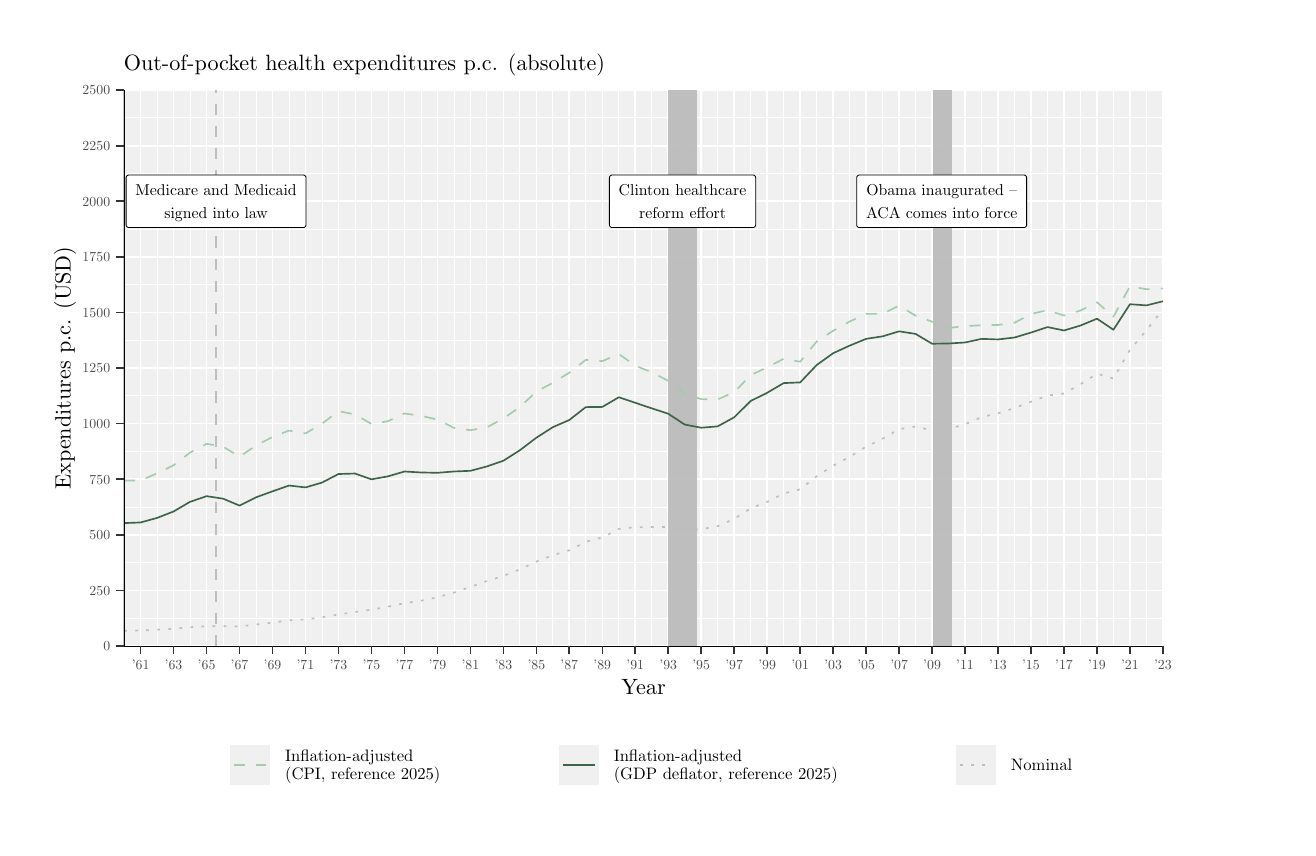
\begin{tikzpicture}[x=1pt,y=1pt]
\definecolor{fillColor}{RGB}{255,255,255}
\path[use as bounding box,fill=fillColor,fill opacity=0.00] (0,0) rectangle (455.30,289.08);
\begin{scope}
\path[clip] (  0.00,  0.00) rectangle (455.30,289.08);
\definecolor{drawColor}{RGB}{255,255,255}
\definecolor{fillColor}{RGB}{255,255,255}

\path[draw=drawColor,line width= 0.6pt,line join=round,line cap=round,fill=fillColor] (  0.00,  0.00) rectangle (455.30,289.08);
\end{scope}
\begin{scope}
\path[clip] (  0.00,  0.00) rectangle (455.30,289.08);
\definecolor{fillColor}{gray}{0.94}

\path[fill=fillColor] ( 34.76, 65.63) rectangle (410.30,266.52);
\definecolor{drawColor}{RGB}{255,255,255}

\path[draw=drawColor,line width= 0.3pt,line join=round] ( 34.76, 75.68) --
	(410.30, 75.68);

\path[draw=drawColor,line width= 0.3pt,line join=round] ( 34.76, 95.77) --
	(410.30, 95.77);

\path[draw=drawColor,line width= 0.3pt,line join=round] ( 34.76,115.85) --
	(410.30,115.85);

\path[draw=drawColor,line width= 0.3pt,line join=round] ( 34.76,135.94) --
	(410.30,135.94);

\path[draw=drawColor,line width= 0.3pt,line join=round] ( 34.76,156.03) --
	(410.30,156.03);

\path[draw=drawColor,line width= 0.3pt,line join=round] ( 34.76,176.12) --
	(410.30,176.12);

\path[draw=drawColor,line width= 0.3pt,line join=round] ( 34.76,196.21) --
	(410.30,196.21);

\path[draw=drawColor,line width= 0.3pt,line join=round] ( 34.76,216.29) --
	(410.30,216.29);

\path[draw=drawColor,line width= 0.3pt,line join=round] ( 34.76,236.38) --
	(410.30,236.38);

\path[draw=drawColor,line width= 0.3pt,line join=round] ( 34.76,256.47) --
	(410.30,256.47);

\path[draw=drawColor,line width= 0.3pt,line join=round] ( 34.85, 65.63) --
	( 34.85,266.52);

\path[draw=drawColor,line width= 0.3pt,line join=round] ( 46.77, 65.63) --
	( 46.77,266.52);

\path[draw=drawColor,line width= 0.3pt,line join=round] ( 58.69, 65.63) --
	( 58.69,266.52);

\path[draw=drawColor,line width= 0.3pt,line join=round] ( 70.60, 65.63) --
	( 70.60,266.52);

\path[draw=drawColor,line width= 0.3pt,line join=round] ( 82.52, 65.63) --
	( 82.52,266.52);

\path[draw=drawColor,line width= 0.3pt,line join=round] ( 94.43, 65.63) --
	( 94.43,266.52);

\path[draw=drawColor,line width= 0.3pt,line join=round] (106.35, 65.63) --
	(106.35,266.52);

\path[draw=drawColor,line width= 0.3pt,line join=round] (118.27, 65.63) --
	(118.27,266.52);

\path[draw=drawColor,line width= 0.3pt,line join=round] (130.18, 65.63) --
	(130.18,266.52);

\path[draw=drawColor,line width= 0.3pt,line join=round] (142.10, 65.63) --
	(142.10,266.52);

\path[draw=drawColor,line width= 0.3pt,line join=round] (154.02, 65.63) --
	(154.02,266.52);

\path[draw=drawColor,line width= 0.3pt,line join=round] (165.93, 65.63) --
	(165.93,266.52);

\path[draw=drawColor,line width= 0.3pt,line join=round] (177.85, 65.63) --
	(177.85,266.52);

\path[draw=drawColor,line width= 0.3pt,line join=round] (189.77, 65.63) --
	(189.77,266.52);

\path[draw=drawColor,line width= 0.3pt,line join=round] (201.68, 65.63) --
	(201.68,266.52);

\path[draw=drawColor,line width= 0.3pt,line join=round] (213.60, 65.63) --
	(213.60,266.52);

\path[draw=drawColor,line width= 0.3pt,line join=round] (225.52, 65.63) --
	(225.52,266.52);

\path[draw=drawColor,line width= 0.3pt,line join=round] (237.43, 65.63) --
	(237.43,266.52);

\path[draw=drawColor,line width= 0.3pt,line join=round] (249.35, 65.63) --
	(249.35,266.52);

\path[draw=drawColor,line width= 0.3pt,line join=round] (261.27, 65.63) --
	(261.27,266.52);

\path[draw=drawColor,line width= 0.3pt,line join=round] (273.18, 65.63) --
	(273.18,266.52);

\path[draw=drawColor,line width= 0.3pt,line join=round] (285.10, 65.63) --
	(285.10,266.52);

\path[draw=drawColor,line width= 0.3pt,line join=round] (297.02, 65.63) --
	(297.02,266.52);

\path[draw=drawColor,line width= 0.3pt,line join=round] (308.93, 65.63) --
	(308.93,266.52);

\path[draw=drawColor,line width= 0.3pt,line join=round] (320.85, 65.63) --
	(320.85,266.52);

\path[draw=drawColor,line width= 0.3pt,line join=round] (332.77, 65.63) --
	(332.77,266.52);

\path[draw=drawColor,line width= 0.3pt,line join=round] (344.68, 65.63) --
	(344.68,266.52);

\path[draw=drawColor,line width= 0.3pt,line join=round] (356.60, 65.63) --
	(356.60,266.52);

\path[draw=drawColor,line width= 0.3pt,line join=round] (368.52, 65.63) --
	(368.52,266.52);

\path[draw=drawColor,line width= 0.3pt,line join=round] (380.43, 65.63) --
	(380.43,266.52);

\path[draw=drawColor,line width= 0.3pt,line join=round] (392.35, 65.63) --
	(392.35,266.52);

\path[draw=drawColor,line width= 0.3pt,line join=round] (404.27, 65.63) --
	(404.27,266.52);

\path[draw=drawColor,line width= 0.6pt,line join=round] ( 34.76, 65.63) --
	(410.30, 65.63);

\path[draw=drawColor,line width= 0.6pt,line join=round] ( 34.76, 85.72) --
	(410.30, 85.72);

\path[draw=drawColor,line width= 0.6pt,line join=round] ( 34.76,105.81) --
	(410.30,105.81);

\path[draw=drawColor,line width= 0.6pt,line join=round] ( 34.76,125.90) --
	(410.30,125.90);

\path[draw=drawColor,line width= 0.6pt,line join=round] ( 34.76,145.99) --
	(410.30,145.99);

\path[draw=drawColor,line width= 0.6pt,line join=round] ( 34.76,166.07) --
	(410.30,166.07);

\path[draw=drawColor,line width= 0.6pt,line join=round] ( 34.76,186.16) --
	(410.30,186.16);

\path[draw=drawColor,line width= 0.6pt,line join=round] ( 34.76,206.25) --
	(410.30,206.25);

\path[draw=drawColor,line width= 0.6pt,line join=round] ( 34.76,226.34) --
	(410.30,226.34);

\path[draw=drawColor,line width= 0.6pt,line join=round] ( 34.76,246.43) --
	(410.30,246.43);

\path[draw=drawColor,line width= 0.6pt,line join=round] ( 34.76,266.52) --
	(410.30,266.52);

\path[draw=drawColor,line width= 0.6pt,line join=round] ( 40.81, 65.63) --
	( 40.81,266.52);

\path[draw=drawColor,line width= 0.6pt,line join=round] ( 52.72, 65.63) --
	( 52.72,266.52);

\path[draw=drawColor,line width= 0.6pt,line join=round] ( 64.65, 65.63) --
	( 64.65,266.52);

\path[draw=drawColor,line width= 0.6pt,line join=round] ( 76.56, 65.63) --
	( 76.56,266.52);

\path[draw=drawColor,line width= 0.6pt,line join=round] ( 88.48, 65.63) --
	( 88.48,266.52);

\path[draw=drawColor,line width= 0.6pt,line join=round] (100.39, 65.63) --
	(100.39,266.52);

\path[draw=drawColor,line width= 0.6pt,line join=round] (112.31, 65.63) --
	(112.31,266.52);

\path[draw=drawColor,line width= 0.6pt,line join=round] (124.22, 65.63) --
	(124.22,266.52);

\path[draw=drawColor,line width= 0.6pt,line join=round] (136.15, 65.63) --
	(136.15,266.52);

\path[draw=drawColor,line width= 0.6pt,line join=round] (148.06, 65.63) --
	(148.06,266.52);

\path[draw=drawColor,line width= 0.6pt,line join=round] (159.98, 65.63) --
	(159.98,266.52);

\path[draw=drawColor,line width= 0.6pt,line join=round] (171.89, 65.63) --
	(171.89,266.52);

\path[draw=drawColor,line width= 0.6pt,line join=round] (183.81, 65.63) --
	(183.81,266.52);

\path[draw=drawColor,line width= 0.6pt,line join=round] (195.72, 65.63) --
	(195.72,266.52);

\path[draw=drawColor,line width= 0.6pt,line join=round] (207.65, 65.63) --
	(207.65,266.52);

\path[draw=drawColor,line width= 0.6pt,line join=round] (219.55, 65.63) --
	(219.55,266.52);

\path[draw=drawColor,line width= 0.6pt,line join=round] (231.48, 65.63) --
	(231.48,266.52);

\path[draw=drawColor,line width= 0.6pt,line join=round] (243.39, 65.63) --
	(243.39,266.52);

\path[draw=drawColor,line width= 0.6pt,line join=round] (255.31, 65.63) --
	(255.31,266.52);

\path[draw=drawColor,line width= 0.6pt,line join=round] (267.22, 65.63) --
	(267.22,266.52);

\path[draw=drawColor,line width= 0.6pt,line join=round] (279.15, 65.63) --
	(279.15,266.52);

\path[draw=drawColor,line width= 0.6pt,line join=round] (291.05, 65.63) --
	(291.05,266.52);

\path[draw=drawColor,line width= 0.6pt,line join=round] (302.98, 65.63) --
	(302.98,266.52);

\path[draw=drawColor,line width= 0.6pt,line join=round] (314.89, 65.63) --
	(314.89,266.52);

\path[draw=drawColor,line width= 0.6pt,line join=round] (326.81, 65.63) --
	(326.81,266.52);

\path[draw=drawColor,line width= 0.6pt,line join=round] (338.72, 65.63) --
	(338.72,266.52);

\path[draw=drawColor,line width= 0.6pt,line join=round] (350.64, 65.63) --
	(350.64,266.52);

\path[draw=drawColor,line width= 0.6pt,line join=round] (362.55, 65.63) --
	(362.55,266.52);

\path[draw=drawColor,line width= 0.6pt,line join=round] (374.48, 65.63) --
	(374.48,266.52);

\path[draw=drawColor,line width= 0.6pt,line join=round] (386.39, 65.63) --
	(386.39,266.52);

\path[draw=drawColor,line width= 0.6pt,line join=round] (398.31, 65.63) --
	(398.31,266.52);

\path[draw=drawColor,line width= 0.6pt,line join=round] (410.22, 65.63) --
	(410.22,266.52);
\definecolor{drawColor}{RGB}{190,190,190}

\path[draw=drawColor,line width= 0.6pt,line join=round] ( 34.84, 65.63) -- ( 34.84,266.52);
\definecolor{fillColor}{RGB}{190,190,190}

\path[fill=fillColor,fill opacity=0.01] (231.48, 65.63) rectangle (241.81,266.52);

\path[fill=fillColor,fill opacity=0.01] (231.48, 65.63) rectangle (241.81,266.52);

\path[fill=fillColor,fill opacity=0.01] (231.48, 65.63) rectangle (241.81,266.52);

\path[fill=fillColor,fill opacity=0.01] (231.48, 65.63) rectangle (241.81,266.52);

\path[fill=fillColor,fill opacity=0.01] (231.48, 65.63) rectangle (241.81,266.52);

\path[fill=fillColor,fill opacity=0.01] (231.48, 65.63) rectangle (241.81,266.52);

\path[fill=fillColor,fill opacity=0.01] (231.48, 65.63) rectangle (241.81,266.52);

\path[fill=fillColor,fill opacity=0.01] (231.48, 65.63) rectangle (241.81,266.52);

\path[fill=fillColor,fill opacity=0.01] (231.48, 65.63) rectangle (241.81,266.52);

\path[fill=fillColor,fill opacity=0.01] (231.48, 65.63) rectangle (241.81,266.52);

\path[fill=fillColor,fill opacity=0.01] (231.48, 65.63) rectangle (241.81,266.52);

\path[fill=fillColor,fill opacity=0.01] (231.48, 65.63) rectangle (241.81,266.52);

\path[fill=fillColor,fill opacity=0.01] (231.48, 65.63) rectangle (241.81,266.52);

\path[fill=fillColor,fill opacity=0.01] (231.48, 65.63) rectangle (241.81,266.52);

\path[fill=fillColor,fill opacity=0.01] (231.48, 65.63) rectangle (241.81,266.52);

\path[fill=fillColor,fill opacity=0.01] (231.48, 65.63) rectangle (241.81,266.52);

\path[fill=fillColor,fill opacity=0.01] (231.48, 65.63) rectangle (241.81,266.52);

\path[fill=fillColor,fill opacity=0.01] (231.48, 65.63) rectangle (241.81,266.52);

\path[fill=fillColor,fill opacity=0.01] (231.48, 65.63) rectangle (241.81,266.52);

\path[fill=fillColor,fill opacity=0.01] (231.48, 65.63) rectangle (241.81,266.52);

\path[fill=fillColor,fill opacity=0.01] (231.48, 65.63) rectangle (241.81,266.52);

\path[fill=fillColor,fill opacity=0.01] (231.48, 65.63) rectangle (241.81,266.52);

\path[fill=fillColor,fill opacity=0.01] (231.48, 65.63) rectangle (241.81,266.52);

\path[fill=fillColor,fill opacity=0.01] (231.48, 65.63) rectangle (241.81,266.52);

\path[fill=fillColor,fill opacity=0.01] (231.48, 65.63) rectangle (241.81,266.52);

\path[fill=fillColor,fill opacity=0.01] (231.48, 65.63) rectangle (241.81,266.52);

\path[fill=fillColor,fill opacity=0.01] (231.48, 65.63) rectangle (241.81,266.52);

\path[fill=fillColor,fill opacity=0.01] (231.48, 65.63) rectangle (241.81,266.52);

\path[fill=fillColor,fill opacity=0.01] (231.48, 65.63) rectangle (241.81,266.52);

\path[fill=fillColor,fill opacity=0.01] (231.48, 65.63) rectangle (241.81,266.52);

\path[fill=fillColor,fill opacity=0.01] (231.48, 65.63) rectangle (241.81,266.52);

\path[fill=fillColor,fill opacity=0.01] (231.48, 65.63) rectangle (241.81,266.52);

\path[fill=fillColor,fill opacity=0.01] (231.48, 65.63) rectangle (241.81,266.52);

\path[fill=fillColor,fill opacity=0.01] (231.48, 65.63) rectangle (241.81,266.52);

\path[fill=fillColor,fill opacity=0.01] (231.48, 65.63) rectangle (241.81,266.52);

\path[fill=fillColor,fill opacity=0.01] (231.48, 65.63) rectangle (241.81,266.52);

\path[fill=fillColor,fill opacity=0.01] (231.48, 65.63) rectangle (241.81,266.52);

\path[fill=fillColor,fill opacity=0.01] (231.48, 65.63) rectangle (241.81,266.52);

\path[fill=fillColor,fill opacity=0.01] (231.48, 65.63) rectangle (241.81,266.52);

\path[fill=fillColor,fill opacity=0.01] (231.48, 65.63) rectangle (241.81,266.52);

\path[fill=fillColor,fill opacity=0.01] (231.48, 65.63) rectangle (241.81,266.52);

\path[fill=fillColor,fill opacity=0.01] (231.48, 65.63) rectangle (241.81,266.52);

\path[fill=fillColor,fill opacity=0.01] (231.48, 65.63) rectangle (241.81,266.52);

\path[fill=fillColor,fill opacity=0.01] (231.48, 65.63) rectangle (241.81,266.52);

\path[fill=fillColor,fill opacity=0.01] (231.48, 65.63) rectangle (241.81,266.52);

\path[fill=fillColor,fill opacity=0.01] (231.48, 65.63) rectangle (241.81,266.52);

\path[fill=fillColor,fill opacity=0.01] (231.48, 65.63) rectangle (241.81,266.52);

\path[fill=fillColor,fill opacity=0.01] (231.48, 65.63) rectangle (241.81,266.52);

\path[fill=fillColor,fill opacity=0.01] (231.48, 65.63) rectangle (241.81,266.52);

\path[fill=fillColor,fill opacity=0.01] (231.48, 65.63) rectangle (241.81,266.52);

\path[fill=fillColor,fill opacity=0.01] (231.48, 65.63) rectangle (241.81,266.52);

\path[fill=fillColor,fill opacity=0.01] (231.48, 65.63) rectangle (241.81,266.52);

\path[fill=fillColor,fill opacity=0.01] (231.48, 65.63) rectangle (241.81,266.52);

\path[fill=fillColor,fill opacity=0.01] (231.48, 65.63) rectangle (241.81,266.52);

\path[fill=fillColor,fill opacity=0.01] (231.48, 65.63) rectangle (241.81,266.52);

\path[fill=fillColor,fill opacity=0.01] (231.48, 65.63) rectangle (241.81,266.52);

\path[fill=fillColor,fill opacity=0.01] (231.48, 65.63) rectangle (241.81,266.52);

\path[fill=fillColor,fill opacity=0.01] (231.48, 65.63) rectangle (241.81,266.52);

\path[fill=fillColor,fill opacity=0.01] (231.48, 65.63) rectangle (241.81,266.52);

\path[fill=fillColor,fill opacity=0.01] (231.48, 65.63) rectangle (241.81,266.52);

\path[fill=fillColor,fill opacity=0.01] (231.48, 65.63) rectangle (241.81,266.52);

\path[fill=fillColor,fill opacity=0.01] (231.48, 65.63) rectangle (241.81,266.52);

\path[fill=fillColor,fill opacity=0.01] (231.48, 65.63) rectangle (241.81,266.52);

\path[fill=fillColor,fill opacity=0.01] (231.48, 65.63) rectangle (241.81,266.52);

\path[fill=fillColor,fill opacity=0.01] (327.12, 65.63) rectangle (334.09,266.52);

\path[fill=fillColor,fill opacity=0.01] (327.12, 65.63) rectangle (334.09,266.52);

\path[fill=fillColor,fill opacity=0.01] (327.12, 65.63) rectangle (334.09,266.52);

\path[fill=fillColor,fill opacity=0.01] (327.12, 65.63) rectangle (334.09,266.52);

\path[fill=fillColor,fill opacity=0.01] (327.12, 65.63) rectangle (334.09,266.52);

\path[fill=fillColor,fill opacity=0.01] (327.12, 65.63) rectangle (334.09,266.52);

\path[fill=fillColor,fill opacity=0.01] (327.12, 65.63) rectangle (334.09,266.52);

\path[fill=fillColor,fill opacity=0.01] (327.12, 65.63) rectangle (334.09,266.52);

\path[fill=fillColor,fill opacity=0.01] (327.12, 65.63) rectangle (334.09,266.52);

\path[fill=fillColor,fill opacity=0.01] (327.12, 65.63) rectangle (334.09,266.52);

\path[fill=fillColor,fill opacity=0.01] (327.12, 65.63) rectangle (334.09,266.52);

\path[fill=fillColor,fill opacity=0.01] (327.12, 65.63) rectangle (334.09,266.52);

\path[fill=fillColor,fill opacity=0.01] (327.12, 65.63) rectangle (334.09,266.52);

\path[fill=fillColor,fill opacity=0.01] (327.12, 65.63) rectangle (334.09,266.52);

\path[fill=fillColor,fill opacity=0.01] (327.12, 65.63) rectangle (334.09,266.52);

\path[fill=fillColor,fill opacity=0.01] (327.12, 65.63) rectangle (334.09,266.52);

\path[fill=fillColor,fill opacity=0.01] (327.12, 65.63) rectangle (334.09,266.52);

\path[fill=fillColor,fill opacity=0.01] (327.12, 65.63) rectangle (334.09,266.52);

\path[fill=fillColor,fill opacity=0.01] (327.12, 65.63) rectangle (334.09,266.52);

\path[fill=fillColor,fill opacity=0.01] (327.12, 65.63) rectangle (334.09,266.52);

\path[fill=fillColor,fill opacity=0.01] (327.12, 65.63) rectangle (334.09,266.52);

\path[fill=fillColor,fill opacity=0.01] (327.12, 65.63) rectangle (334.09,266.52);

\path[fill=fillColor,fill opacity=0.01] (327.12, 65.63) rectangle (334.09,266.52);

\path[fill=fillColor,fill opacity=0.01] (327.12, 65.63) rectangle (334.09,266.52);

\path[fill=fillColor,fill opacity=0.01] (327.12, 65.63) rectangle (334.09,266.52);

\path[fill=fillColor,fill opacity=0.01] (327.12, 65.63) rectangle (334.09,266.52);

\path[fill=fillColor,fill opacity=0.01] (327.12, 65.63) rectangle (334.09,266.52);

\path[fill=fillColor,fill opacity=0.01] (327.12, 65.63) rectangle (334.09,266.52);

\path[fill=fillColor,fill opacity=0.01] (327.12, 65.63) rectangle (334.09,266.52);

\path[fill=fillColor,fill opacity=0.01] (327.12, 65.63) rectangle (334.09,266.52);

\path[fill=fillColor,fill opacity=0.01] (327.12, 65.63) rectangle (334.09,266.52);

\path[fill=fillColor,fill opacity=0.01] (327.12, 65.63) rectangle (334.09,266.52);

\path[fill=fillColor,fill opacity=0.01] (327.12, 65.63) rectangle (334.09,266.52);

\path[fill=fillColor,fill opacity=0.01] (327.12, 65.63) rectangle (334.09,266.52);

\path[fill=fillColor,fill opacity=0.01] (327.12, 65.63) rectangle (334.09,266.52);

\path[fill=fillColor,fill opacity=0.01] (327.12, 65.63) rectangle (334.09,266.52);

\path[fill=fillColor,fill opacity=0.01] (327.12, 65.63) rectangle (334.09,266.52);

\path[fill=fillColor,fill opacity=0.01] (327.12, 65.63) rectangle (334.09,266.52);

\path[fill=fillColor,fill opacity=0.01] (327.12, 65.63) rectangle (334.09,266.52);

\path[fill=fillColor,fill opacity=0.01] (327.12, 65.63) rectangle (334.09,266.52);

\path[fill=fillColor,fill opacity=0.01] (327.12, 65.63) rectangle (334.09,266.52);

\path[fill=fillColor,fill opacity=0.01] (327.12, 65.63) rectangle (334.09,266.52);

\path[fill=fillColor,fill opacity=0.01] (327.12, 65.63) rectangle (334.09,266.52);

\path[fill=fillColor,fill opacity=0.01] (327.12, 65.63) rectangle (334.09,266.52);

\path[fill=fillColor,fill opacity=0.01] (327.12, 65.63) rectangle (334.09,266.52);

\path[fill=fillColor,fill opacity=0.01] (327.12, 65.63) rectangle (334.09,266.52);

\path[fill=fillColor,fill opacity=0.01] (327.12, 65.63) rectangle (334.09,266.52);

\path[fill=fillColor,fill opacity=0.01] (327.12, 65.63) rectangle (334.09,266.52);

\path[fill=fillColor,fill opacity=0.01] (327.12, 65.63) rectangle (334.09,266.52);

\path[fill=fillColor,fill opacity=0.01] (327.12, 65.63) rectangle (334.09,266.52);

\path[fill=fillColor,fill opacity=0.01] (327.12, 65.63) rectangle (334.09,266.52);

\path[fill=fillColor,fill opacity=0.01] (327.12, 65.63) rectangle (334.09,266.52);

\path[fill=fillColor,fill opacity=0.01] (327.12, 65.63) rectangle (334.09,266.52);

\path[fill=fillColor,fill opacity=0.01] (327.12, 65.63) rectangle (334.09,266.52);

\path[fill=fillColor,fill opacity=0.01] (327.12, 65.63) rectangle (334.09,266.52);

\path[fill=fillColor,fill opacity=0.01] (327.12, 65.63) rectangle (334.09,266.52);

\path[fill=fillColor,fill opacity=0.01] (327.12, 65.63) rectangle (334.09,266.52);

\path[fill=fillColor,fill opacity=0.01] (327.12, 65.63) rectangle (334.09,266.52);

\path[fill=fillColor,fill opacity=0.01] (327.12, 65.63) rectangle (334.09,266.52);

\path[fill=fillColor,fill opacity=0.01] (327.12, 65.63) rectangle (334.09,266.52);

\path[fill=fillColor,fill opacity=0.01] (327.12, 65.63) rectangle (334.09,266.52);

\path[fill=fillColor,fill opacity=0.01] (327.12, 65.63) rectangle (334.09,266.52);

\path[fill=fillColor,fill opacity=0.01] (327.12, 65.63) rectangle (334.09,266.52);

\path[fill=fillColor,fill opacity=0.01] (327.12, 65.63) rectangle (334.09,266.52);

\path[draw=drawColor,line width= 0.6pt,dash pattern=on 4pt off 4pt ,line join=round] ( 68.07, 65.63) -- ( 68.07,266.52);
\definecolor{drawColor}{RGB}{0,0,0}
\definecolor{fillColor}{RGB}{255,255,255}

\path[draw=drawColor,line width= 0.3pt,line join=round,line cap=round,fill=fillColor] ( 36.59,216.85) --
	( 99.56,216.85) --
	( 99.52,216.86) --
	( 99.68,216.86) --
	( 99.85,216.90) --
	(100.00,216.95) --
	(100.14,217.04) --
	(100.27,217.14) --
	(100.38,217.27) --
	(100.47,217.41) --
	(100.54,217.56) --
	(100.58,217.72) --
	(100.59,217.88) --
	(100.59,217.88) --
	(100.59,234.79) --
	(100.59,234.79) --
	(100.58,234.96) --
	(100.54,235.12) --
	(100.47,235.27) --
	(100.38,235.41) --
	(100.27,235.54) --
	(100.14,235.64) --
	(100.00,235.72) --
	( 99.85,235.78) --
	( 99.68,235.82) --
	( 99.56,235.82) --
	( 36.59,235.82) --
	( 36.71,235.82) --
	( 36.54,235.82) --
	( 36.38,235.80) --
	( 36.22,235.76) --
	( 36.07,235.69) --
	( 35.94,235.59) --
	( 35.82,235.48) --
	( 35.72,235.34) --
	( 35.64,235.20) --
	( 35.59,235.04) --
	( 35.56,234.88) --
	( 35.56,234.79) --
	( 35.56,217.88) --
	( 35.56,217.97) --
	( 35.56,217.80) --
	( 35.59,217.64) --
	( 35.64,217.48) --
	( 35.72,217.33) --
	( 35.82,217.20) --
	( 35.94,217.09) --
	( 36.07,216.99) --
	( 36.22,216.92) --
	( 36.38,216.88) --
	( 36.54,216.86) --
	cycle;
\end{scope}
\begin{scope}
\path[clip] (  0.00,  0.00) rectangle (455.30,289.08);
\definecolor{drawColor}{RGB}{0,0,0}

\node[text=drawColor,anchor=base,inner sep=0pt, outer sep=0pt, scale=  0.57] at ( 68.07,228.48) {Medicare and Medicaid };

\node[text=drawColor,anchor=base,inner sep=0pt, outer sep=0pt, scale=  0.57] at ( 68.07,220.28) { signed into law};
\end{scope}
\begin{scope}
\path[clip] (  0.00,  0.00) rectangle (455.30,289.08);
\definecolor{drawColor}{RGB}{0,0,0}
\definecolor{fillColor}{RGB}{255,255,255}

\path[draw=drawColor,line width= 0.3pt,line join=round,line cap=round,fill=fillColor] (211.23,216.85) --
	(262.04,216.85) --
	(262.00,216.86) --
	(262.16,216.86) --
	(262.32,216.90) --
	(262.48,216.95) --
	(262.62,217.04) --
	(262.75,217.14) --
	(262.86,217.27) --
	(262.95,217.41) --
	(263.01,217.56) --
	(263.05,217.72) --
	(263.07,217.88) --
	(263.07,217.88) --
	(263.07,234.79) --
	(263.07,234.79) --
	(263.05,234.96) --
	(263.01,235.12) --
	(262.95,235.27) --
	(262.86,235.41) --
	(262.75,235.54) --
	(262.62,235.64) --
	(262.48,235.72) --
	(262.32,235.78) --
	(262.16,235.82) --
	(262.04,235.82) --
	(211.23,235.82) --
	(211.36,235.82) --
	(211.19,235.82) --
	(211.03,235.80) --
	(210.87,235.76) --
	(210.72,235.69) --
	(210.58,235.59) --
	(210.46,235.48) --
	(210.36,235.34) --
	(210.29,235.20) --
	(210.23,235.04) --
	(210.21,234.88) --
	(210.20,234.79) --
	(210.20,217.88) --
	(210.21,217.97) --
	(210.21,217.80) --
	(210.23,217.64) --
	(210.29,217.48) --
	(210.36,217.33) --
	(210.46,217.20) --
	(210.58,217.09) --
	(210.72,216.99) --
	(210.87,216.92) --
	(211.03,216.88) --
	(211.19,216.86) --
	cycle;
\end{scope}
\begin{scope}
\path[clip] (  0.00,  0.00) rectangle (455.30,289.08);
\definecolor{drawColor}{RGB}{0,0,0}

\node[text=drawColor,anchor=base,inner sep=0pt, outer sep=0pt, scale=  0.57] at (236.63,228.48) {Clinton healthcare };

\node[text=drawColor,anchor=base,inner sep=0pt, outer sep=0pt, scale=  0.57] at (236.63,220.28) { reform effort};
\end{scope}
\begin{scope}
\path[clip] (  0.00,  0.00) rectangle (455.30,289.08);
\definecolor{drawColor}{RGB}{0,0,0}
\definecolor{fillColor}{RGB}{255,255,255}

\path[draw=drawColor,line width= 0.3pt,line join=round,line cap=round,fill=fillColor] (300.58,216.85) --
	(359.96,216.85) --
	(359.91,216.86) --
	(360.08,216.86) --
	(360.24,216.90) --
	(360.40,216.95) --
	(360.54,217.04) --
	(360.67,217.14) --
	(360.78,217.27) --
	(360.87,217.41) --
	(360.93,217.56) --
	(360.97,217.72) --
	(360.98,217.88) --
	(360.98,217.88) --
	(360.98,234.79) --
	(360.98,234.79) --
	(360.97,234.96) --
	(360.93,235.12) --
	(360.87,235.27) --
	(360.78,235.41) --
	(360.67,235.54) --
	(360.54,235.64) --
	(360.40,235.72) --
	(360.24,235.78) --
	(360.08,235.82) --
	(359.96,235.82) --
	(300.58,235.82) --
	(300.71,235.82) --
	(300.54,235.82) --
	(300.38,235.80) --
	(300.22,235.76) --
	(300.07,235.69) --
	(299.93,235.59) --
	(299.81,235.48) --
	(299.72,235.34) --
	(299.64,235.20) --
	(299.59,235.04) --
	(299.56,234.88) --
	(299.56,234.79) --
	(299.56,217.88) --
	(299.56,217.97) --
	(299.56,217.80) --
	(299.59,217.64) --
	(299.64,217.48) --
	(299.72,217.33) --
	(299.81,217.20) --
	(299.93,217.09) --
	(300.07,216.99) --
	(300.22,216.92) --
	(300.38,216.88) --
	(300.54,216.86) --
	cycle;
\end{scope}
\begin{scope}
\path[clip] (  0.00,  0.00) rectangle (455.30,289.08);
\definecolor{drawColor}{RGB}{0,0,0}

\node[text=drawColor,anchor=base,inner sep=0pt, outer sep=0pt, scale=  0.57] at (330.27,228.48) {Obama inaugurated -- };

\node[text=drawColor,anchor=base,inner sep=0pt, outer sep=0pt, scale=  0.57] at (330.27,220.28) { ACA comes into force};
\end{scope}
\begin{scope}
\path[clip] (  0.00,  0.00) rectangle (455.30,289.08);
\definecolor{drawColor}{RGB}{190,190,190}

\path[draw=drawColor,line width= 0.6pt,dash pattern=on 1pt off 3pt ,line join=round] ( 34.84, 71.15) --
	( 40.81, 71.24) --
	( 46.77, 71.53) --
	( 52.72, 71.89) --
	( 58.68, 72.43) --
	( 64.65, 72.81) --
	( 70.60, 72.85) --
	( 76.56, 72.72) --
	( 82.51, 73.42) --
	( 88.48, 74.10) --
	( 94.43, 74.90) --
	(100.39, 75.26) --
	(106.34, 76.03) --
	(112.31, 77.02) --
	(118.27, 77.91) --
	(124.22, 78.80) --
	(130.18, 79.85) --
	(136.15, 81.11) --
	(142.10, 82.00) --
	(148.06, 83.23) --
	(154.01, 84.94) --
	(159.98, 86.99) --
	(165.93, 89.09) --
	(171.89, 90.95) --
	(177.84, 93.34) --
	(183.81, 96.16) --
	(189.77, 98.45) --
	(195.72,100.21) --
	(201.68,103.30) --
	(207.65,104.88) --
	(213.60,107.95) --
	(219.55,108.56) --
	(225.51,108.64) --
	(231.48,108.65) --
	(237.43,107.56) --
	(243.39,107.85) --
	(249.34,108.95) --
	(255.31,111.59) --
	(261.27,115.42) --
	(267.22,117.73) --
	(273.18,120.79) --
	(279.15,122.27) --
	(285.10,126.99) --
	(291.05,130.79) --
	(297.01,133.99) --
	(302.98,137.68) --
	(308.93,140.58) --
	(314.89,144.01) --
	(320.84,144.95) --
	(326.81,143.53) --
	(332.77,144.03) --
	(338.72,145.78) --
	(344.67,148.34) --
	(350.64,149.74) --
	(356.60,151.64) --
	(362.55,153.92) --
	(368.51,156.14) --
	(374.48,156.91) --
	(380.43,160.23) --
	(386.39,164.06) --
	(392.34,162.29) --
	(398.31,172.67) --
	(404.27,179.75) --
	(410.22,187.29);
\definecolor{drawColor}{RGB}{164,203,174}

\path[draw=drawColor,line width= 0.6pt,dash pattern=on 4pt off 4pt ,line join=round] ( 34.84,125.48) --
	( 40.81,125.43) --
	( 46.77,128.05) --
	( 52.72,130.96) --
	( 58.68,135.53) --
	( 64.65,138.71) --
	( 70.60,137.69) --
	( 76.56,134.04) --
	( 82.51,138.13) --
	( 88.48,141.17) --
	( 94.43,143.48) --
	(100.39,142.46) --
	(106.34,145.95) --
	(112.31,150.51) --
	(118.27,149.33) --
	(124.22,145.89) --
	(130.18,146.87) --
	(136.15,149.66) --
	(142.10,148.84) --
	(148.06,147.48) --
	(154.01,144.46) --
	(159.98,143.62) --
	(165.93,144.66) --
	(171.89,147.85) --
	(177.84,152.02) --
	(183.81,157.56) --
	(189.77,160.76) --
	(195.72,164.40) --
	(201.68,169.04) --
	(207.65,168.59) --
	(213.60,171.15) --
	(219.55,166.95) --
	(225.51,164.55) --
	(231.48,161.46) --
	(237.43,156.73) --
	(243.39,154.86) --
	(249.34,154.75) --
	(255.31,157.40) --
	(261.27,163.50) --
	(267.22,166.36) --
	(273.18,169.43) --
	(279.15,168.38) --
	(285.10,175.69) --
	(291.05,179.55) --
	(297.01,182.89) --
	(302.98,185.64) --
	(308.93,185.70) --
	(314.89,188.64) --
	(320.84,185.00) --
	(326.81,182.84) --
	(332.77,180.56) --
	(338.72,181.24) --
	(344.67,181.55) --
	(350.64,181.66) --
	(356.60,182.44) --
	(362.55,185.64) --
	(368.51,186.99) --
	(374.48,185.04) --
	(380.43,186.87) --
	(386.39,189.86) --
	(392.34,184.65) --
	(398.31,195.62) --
	(404.27,194.57) --
	(410.22,194.81);
\definecolor{drawColor}{RGB}{60,100,75}

\path[draw=drawColor,line width= 0.6pt,line join=round] ( 34.84,110.06) --
	( 40.81,110.28) --
	( 46.77,111.94) --
	( 52.72,114.25) --
	( 58.68,117.75) --
	( 64.65,119.79) --
	( 70.60,118.89) --
	( 76.56,116.38) --
	( 82.51,119.37) --
	( 88.48,121.54) --
	( 94.43,123.63) --
	(100.39,122.95) --
	(106.34,124.69) --
	(112.31,127.79) --
	(118.27,127.97) --
	(124.22,125.87) --
	(130.18,126.95) --
	(136.15,128.70) --
	(142.10,128.35) --
	(148.06,128.23) --
	(154.01,128.71) --
	(159.98,128.95) --
	(165.93,130.53) --
	(171.89,132.59) --
	(177.84,136.37) --
	(183.81,140.91) --
	(189.77,144.72) --
	(195.72,147.32) --
	(201.68,151.97) --
	(207.65,152.04) --
	(213.60,155.52) --
	(219.55,153.53) --
	(225.51,151.53) --
	(231.48,149.57) --
	(237.43,145.66) --
	(243.39,144.52) --
	(249.34,145.01) --
	(255.31,148.30) --
	(261.27,154.20) --
	(267.22,157.15) --
	(273.18,160.65) --
	(279.15,160.89) --
	(285.10,167.17) --
	(291.05,171.44) --
	(297.01,174.18) --
	(302.98,176.64) --
	(308.93,177.54) --
	(314.89,179.35) --
	(320.84,178.42) --
	(326.81,174.87) --
	(332.77,174.96) --
	(338.72,175.32) --
	(344.67,176.62) --
	(350.64,176.42) --
	(356.60,177.12) --
	(362.55,178.91) --
	(368.51,180.89) --
	(374.48,179.66) --
	(380.43,181.45) --
	(386.39,183.91) --
	(392.34,179.93) --
	(398.31,189.15) --
	(404.27,188.72) --
	(410.22,190.21);
\end{scope}
\begin{scope}
\path[clip] (  0.00,  0.00) rectangle (455.30,289.08);
\definecolor{drawColor}{RGB}{0,0,0}

\path[draw=drawColor,line width= 0.2pt,line join=round] ( 34.76, 65.63) --
	( 34.76,266.52);
\end{scope}
\begin{scope}
\path[clip] (  0.00,  0.00) rectangle (455.30,289.08);
\definecolor{drawColor}{gray}{0.30}

\node[text=drawColor,anchor=base east,inner sep=0pt, outer sep=0pt, scale=  0.50] at ( 29.81, 63.91) {0};

\node[text=drawColor,anchor=base east,inner sep=0pt, outer sep=0pt, scale=  0.50] at ( 29.81, 84.00) {250};

\node[text=drawColor,anchor=base east,inner sep=0pt, outer sep=0pt, scale=  0.50] at ( 29.81,104.09) {500};

\node[text=drawColor,anchor=base east,inner sep=0pt, outer sep=0pt, scale=  0.50] at ( 29.81,124.18) {750};

\node[text=drawColor,anchor=base east,inner sep=0pt, outer sep=0pt, scale=  0.50] at ( 29.81,144.26) {1000};

\node[text=drawColor,anchor=base east,inner sep=0pt, outer sep=0pt, scale=  0.50] at ( 29.81,164.35) {1250};

\node[text=drawColor,anchor=base east,inner sep=0pt, outer sep=0pt, scale=  0.50] at ( 29.81,184.44) {1500};

\node[text=drawColor,anchor=base east,inner sep=0pt, outer sep=0pt, scale=  0.50] at ( 29.81,204.53) {1750};

\node[text=drawColor,anchor=base east,inner sep=0pt, outer sep=0pt, scale=  0.50] at ( 29.81,224.62) {2000};

\node[text=drawColor,anchor=base east,inner sep=0pt, outer sep=0pt, scale=  0.50] at ( 29.81,244.71) {2250};

\node[text=drawColor,anchor=base east,inner sep=0pt, outer sep=0pt, scale=  0.50] at ( 29.81,264.79) {2500};
\end{scope}
\begin{scope}
\path[clip] (  0.00,  0.00) rectangle (455.30,289.08);
\definecolor{drawColor}{gray}{0.20}

\path[draw=drawColor,line width= 0.6pt,line join=round] ( 32.01, 65.63) --
	( 34.76, 65.63);

\path[draw=drawColor,line width= 0.6pt,line join=round] ( 32.01, 85.72) --
	( 34.76, 85.72);

\path[draw=drawColor,line width= 0.6pt,line join=round] ( 32.01,105.81) --
	( 34.76,105.81);

\path[draw=drawColor,line width= 0.6pt,line join=round] ( 32.01,125.90) --
	( 34.76,125.90);

\path[draw=drawColor,line width= 0.6pt,line join=round] ( 32.01,145.99) --
	( 34.76,145.99);

\path[draw=drawColor,line width= 0.6pt,line join=round] ( 32.01,166.07) --
	( 34.76,166.07);

\path[draw=drawColor,line width= 0.6pt,line join=round] ( 32.01,186.16) --
	( 34.76,186.16);

\path[draw=drawColor,line width= 0.6pt,line join=round] ( 32.01,206.25) --
	( 34.76,206.25);

\path[draw=drawColor,line width= 0.6pt,line join=round] ( 32.01,226.34) --
	( 34.76,226.34);

\path[draw=drawColor,line width= 0.6pt,line join=round] ( 32.01,246.43) --
	( 34.76,246.43);

\path[draw=drawColor,line width= 0.6pt,line join=round] ( 32.01,266.52) --
	( 34.76,266.52);
\end{scope}
\begin{scope}
\path[clip] (  0.00,  0.00) rectangle (455.30,289.08);
\definecolor{drawColor}{RGB}{0,0,0}

\path[draw=drawColor,line width= 0.2pt,line join=round] ( 34.76, 65.63) --
	(410.30, 65.63);
\end{scope}
\begin{scope}
\path[clip] (  0.00,  0.00) rectangle (455.30,289.08);
\definecolor{drawColor}{gray}{0.20}

\path[draw=drawColor,line width= 0.6pt,line join=round] ( 40.81, 62.88) --
	( 40.81, 65.63);

\path[draw=drawColor,line width= 0.6pt,line join=round] ( 52.72, 62.88) --
	( 52.72, 65.63);

\path[draw=drawColor,line width= 0.6pt,line join=round] ( 64.65, 62.88) --
	( 64.65, 65.63);

\path[draw=drawColor,line width= 0.6pt,line join=round] ( 76.56, 62.88) --
	( 76.56, 65.63);

\path[draw=drawColor,line width= 0.6pt,line join=round] ( 88.48, 62.88) --
	( 88.48, 65.63);

\path[draw=drawColor,line width= 0.6pt,line join=round] (100.39, 62.88) --
	(100.39, 65.63);

\path[draw=drawColor,line width= 0.6pt,line join=round] (112.31, 62.88) --
	(112.31, 65.63);

\path[draw=drawColor,line width= 0.6pt,line join=round] (124.22, 62.88) --
	(124.22, 65.63);

\path[draw=drawColor,line width= 0.6pt,line join=round] (136.15, 62.88) --
	(136.15, 65.63);

\path[draw=drawColor,line width= 0.6pt,line join=round] (148.06, 62.88) --
	(148.06, 65.63);

\path[draw=drawColor,line width= 0.6pt,line join=round] (159.98, 62.88) --
	(159.98, 65.63);

\path[draw=drawColor,line width= 0.6pt,line join=round] (171.89, 62.88) --
	(171.89, 65.63);

\path[draw=drawColor,line width= 0.6pt,line join=round] (183.81, 62.88) --
	(183.81, 65.63);

\path[draw=drawColor,line width= 0.6pt,line join=round] (195.72, 62.88) --
	(195.72, 65.63);

\path[draw=drawColor,line width= 0.6pt,line join=round] (207.65, 62.88) --
	(207.65, 65.63);

\path[draw=drawColor,line width= 0.6pt,line join=round] (219.55, 62.88) --
	(219.55, 65.63);

\path[draw=drawColor,line width= 0.6pt,line join=round] (231.48, 62.88) --
	(231.48, 65.63);

\path[draw=drawColor,line width= 0.6pt,line join=round] (243.39, 62.88) --
	(243.39, 65.63);

\path[draw=drawColor,line width= 0.6pt,line join=round] (255.31, 62.88) --
	(255.31, 65.63);

\path[draw=drawColor,line width= 0.6pt,line join=round] (267.22, 62.88) --
	(267.22, 65.63);

\path[draw=drawColor,line width= 0.6pt,line join=round] (279.15, 62.88) --
	(279.15, 65.63);

\path[draw=drawColor,line width= 0.6pt,line join=round] (291.05, 62.88) --
	(291.05, 65.63);

\path[draw=drawColor,line width= 0.6pt,line join=round] (302.98, 62.88) --
	(302.98, 65.63);

\path[draw=drawColor,line width= 0.6pt,line join=round] (314.89, 62.88) --
	(314.89, 65.63);

\path[draw=drawColor,line width= 0.6pt,line join=round] (326.81, 62.88) --
	(326.81, 65.63);

\path[draw=drawColor,line width= 0.6pt,line join=round] (338.72, 62.88) --
	(338.72, 65.63);

\path[draw=drawColor,line width= 0.6pt,line join=round] (350.64, 62.88) --
	(350.64, 65.63);

\path[draw=drawColor,line width= 0.6pt,line join=round] (362.55, 62.88) --
	(362.55, 65.63);

\path[draw=drawColor,line width= 0.6pt,line join=round] (374.48, 62.88) --
	(374.48, 65.63);

\path[draw=drawColor,line width= 0.6pt,line join=round] (386.39, 62.88) --
	(386.39, 65.63);

\path[draw=drawColor,line width= 0.6pt,line join=round] (398.31, 62.88) --
	(398.31, 65.63);

\path[draw=drawColor,line width= 0.6pt,line join=round] (410.22, 62.88) --
	(410.22, 65.63);
\end{scope}
\begin{scope}
\path[clip] (  0.00,  0.00) rectangle (455.30,289.08);
\definecolor{drawColor}{gray}{0.30}

\node[text=drawColor,anchor=base,inner sep=0pt, outer sep=0pt, scale=  0.50] at ( 40.81, 57.24) {'61};

\node[text=drawColor,anchor=base,inner sep=0pt, outer sep=0pt, scale=  0.50] at ( 52.72, 57.24) {'63};

\node[text=drawColor,anchor=base,inner sep=0pt, outer sep=0pt, scale=  0.50] at ( 64.65, 57.24) {'65};

\node[text=drawColor,anchor=base,inner sep=0pt, outer sep=0pt, scale=  0.50] at ( 76.56, 57.24) {'67};

\node[text=drawColor,anchor=base,inner sep=0pt, outer sep=0pt, scale=  0.50] at ( 88.48, 57.24) {'69};

\node[text=drawColor,anchor=base,inner sep=0pt, outer sep=0pt, scale=  0.50] at (100.39, 57.24) {'71};

\node[text=drawColor,anchor=base,inner sep=0pt, outer sep=0pt, scale=  0.50] at (112.31, 57.24) {'73};

\node[text=drawColor,anchor=base,inner sep=0pt, outer sep=0pt, scale=  0.50] at (124.22, 57.24) {'75};

\node[text=drawColor,anchor=base,inner sep=0pt, outer sep=0pt, scale=  0.50] at (136.15, 57.24) {'77};

\node[text=drawColor,anchor=base,inner sep=0pt, outer sep=0pt, scale=  0.50] at (148.06, 57.24) {'79};

\node[text=drawColor,anchor=base,inner sep=0pt, outer sep=0pt, scale=  0.50] at (159.98, 57.24) {'81};

\node[text=drawColor,anchor=base,inner sep=0pt, outer sep=0pt, scale=  0.50] at (171.89, 57.24) {'83};

\node[text=drawColor,anchor=base,inner sep=0pt, outer sep=0pt, scale=  0.50] at (183.81, 57.24) {'85};

\node[text=drawColor,anchor=base,inner sep=0pt, outer sep=0pt, scale=  0.50] at (195.72, 57.24) {'87};

\node[text=drawColor,anchor=base,inner sep=0pt, outer sep=0pt, scale=  0.50] at (207.65, 57.24) {'89};

\node[text=drawColor,anchor=base,inner sep=0pt, outer sep=0pt, scale=  0.50] at (219.55, 57.24) {'91};

\node[text=drawColor,anchor=base,inner sep=0pt, outer sep=0pt, scale=  0.50] at (231.48, 57.24) {'93};

\node[text=drawColor,anchor=base,inner sep=0pt, outer sep=0pt, scale=  0.50] at (243.39, 57.24) {'95};

\node[text=drawColor,anchor=base,inner sep=0pt, outer sep=0pt, scale=  0.50] at (255.31, 57.24) {'97};

\node[text=drawColor,anchor=base,inner sep=0pt, outer sep=0pt, scale=  0.50] at (267.22, 57.24) {'99};

\node[text=drawColor,anchor=base,inner sep=0pt, outer sep=0pt, scale=  0.50] at (279.15, 57.24) {'01};

\node[text=drawColor,anchor=base,inner sep=0pt, outer sep=0pt, scale=  0.50] at (291.05, 57.24) {'03};

\node[text=drawColor,anchor=base,inner sep=0pt, outer sep=0pt, scale=  0.50] at (302.98, 57.24) {'05};

\node[text=drawColor,anchor=base,inner sep=0pt, outer sep=0pt, scale=  0.50] at (314.89, 57.24) {'07};

\node[text=drawColor,anchor=base,inner sep=0pt, outer sep=0pt, scale=  0.50] at (326.81, 57.24) {'09};

\node[text=drawColor,anchor=base,inner sep=0pt, outer sep=0pt, scale=  0.50] at (338.72, 57.24) {'11};

\node[text=drawColor,anchor=base,inner sep=0pt, outer sep=0pt, scale=  0.50] at (350.64, 57.24) {'13};

\node[text=drawColor,anchor=base,inner sep=0pt, outer sep=0pt, scale=  0.50] at (362.55, 57.24) {'15};

\node[text=drawColor,anchor=base,inner sep=0pt, outer sep=0pt, scale=  0.50] at (374.48, 57.24) {'17};

\node[text=drawColor,anchor=base,inner sep=0pt, outer sep=0pt, scale=  0.50] at (386.39, 57.24) {'19};

\node[text=drawColor,anchor=base,inner sep=0pt, outer sep=0pt, scale=  0.50] at (398.31, 57.24) {'21};

\node[text=drawColor,anchor=base,inner sep=0pt, outer sep=0pt, scale=  0.50] at (410.22, 57.24) {'23};
\end{scope}
\begin{scope}
\path[clip] (  0.00,  0.00) rectangle (455.30,289.08);
\definecolor{drawColor}{RGB}{0,0,0}

\node[text=drawColor,anchor=base,inner sep=0pt, outer sep=0pt, scale=  0.80] at (222.53, 48.01) {Year};
\end{scope}
\begin{scope}
\path[clip] (  0.00,  0.00) rectangle (455.30,289.08);
\definecolor{drawColor}{RGB}{0,0,0}

\node[text=drawColor,rotate= 90.00,anchor=base,inner sep=0pt, outer sep=0pt, scale=  0.80] at ( 15.51,166.07) {Expenditures p.c. (USD)};
\end{scope}
\begin{scope}
\path[clip] (  0.00,  0.00) rectangle (455.30,289.08);
\definecolor{fillColor}{RGB}{255,255,255}

\path[fill=fillColor] ( 62.09, 10.00) rectangle (382.98, 35.45);
\end{scope}
\begin{scope}
\path[clip] (  0.00,  0.00) rectangle (455.30,289.08);
\definecolor{fillColor}{gray}{0.94}

\path[fill=fillColor] ( 73.09, 15.50) rectangle ( 87.54, 29.95);
\end{scope}
\begin{scope}
\path[clip] (  0.00,  0.00) rectangle (455.30,289.08);
\definecolor{drawColor}{RGB}{164,203,174}

\path[draw=drawColor,line width= 0.6pt,dash pattern=on 4pt off 4pt ,line join=round] ( 74.53, 22.73) -- ( 86.09, 22.73);
\end{scope}
\begin{scope}
\path[clip] (  0.00,  0.00) rectangle (455.30,289.08);
\definecolor{fillColor}{gray}{0.94}

\path[fill=fillColor] (191.82, 15.50) rectangle (206.28, 29.95);
\end{scope}
\begin{scope}
\path[clip] (  0.00,  0.00) rectangle (455.30,289.08);
\definecolor{drawColor}{RGB}{60,100,75}

\path[draw=drawColor,line width= 0.6pt,line join=round] (193.27, 22.73) -- (204.83, 22.73);
\end{scope}
\begin{scope}
\path[clip] (  0.00,  0.00) rectangle (455.30,289.08);
\definecolor{fillColor}{gray}{0.94}

\path[fill=fillColor] (335.36, 15.50) rectangle (349.82, 29.95);
\end{scope}
\begin{scope}
\path[clip] (  0.00,  0.00) rectangle (455.30,289.08);
\definecolor{drawColor}{RGB}{190,190,190}

\path[draw=drawColor,line width= 0.6pt,dash pattern=on 1pt off 3pt ,line join=round] (336.81, 22.73) -- (348.37, 22.73);
\end{scope}
\begin{scope}
\path[clip] (  0.00,  0.00) rectangle (455.30,289.08);
\definecolor{drawColor}{RGB}{0,0,0}

\node[text=drawColor,anchor=base west,inner sep=0pt, outer sep=0pt, scale=  0.60] at ( 93.04, 23.90) {Inflation-adjusted };

\node[text=drawColor,anchor=base west,inner sep=0pt, outer sep=0pt, scale=  0.60] at ( 93.04, 17.42) { (CPI, reference 2025)};
\end{scope}
\begin{scope}
\path[clip] (  0.00,  0.00) rectangle (455.30,289.08);
\definecolor{drawColor}{RGB}{0,0,0}

\node[text=drawColor,anchor=base west,inner sep=0pt, outer sep=0pt, scale=  0.60] at (211.78, 23.90) {Inflation-adjusted  };

\node[text=drawColor,anchor=base west,inner sep=0pt, outer sep=0pt, scale=  0.60] at (211.78, 17.42) { (GDP deflator, reference 2025)};
\end{scope}
\begin{scope}
\path[clip] (  0.00,  0.00) rectangle (455.30,289.08);
\definecolor{drawColor}{RGB}{0,0,0}

\node[text=drawColor,anchor=base west,inner sep=0pt, outer sep=0pt, scale=  0.60] at (355.32, 20.66) {Nominal};
\end{scope}
\begin{scope}
\path[clip] (  0.00,  0.00) rectangle (455.30,289.08);
\definecolor{drawColor}{RGB}{0,0,0}

\node[text=drawColor,anchor=base west,inner sep=0pt, outer sep=0pt, scale=  0.80] at ( 34.76,273.57) {Out-of-pocket health expenditures p.c. (absolute)};
\end{scope}
\end{tikzpicture}
